\documentclass[fr]{../../../../../../eplexam}

\usepackage{../../../../../../eplchem}
\usepackage{../../../../../../eplunits}

\newcommand{\potstd}[1]{E\std_{\text{éq},\text{#1}}}
\newcommand{\potstdce}{\potstd{cell}}
\newcommand{\potstdca}{\potstd{cathode}}
\newcommand{\potstdan}{\potstd{anode}}

\hypertitle{Chimie et chimie physique}{3}{FSAB}{1302}{2016}{Août}{All}
{Louis Devillez}
{Hervé Jeanmart et Joris Proost}

\section{Question 1}
Des expériences en laboratoire ont permis de démontrer qu'une réaction chimique en phase gazeuse se déroule suivant un mécanisme réactionnel à trois étapes:

\begin{itemize} 
	\item \'Etape 1: \ce{Cl2} = 2 \ce{Cl} (rapide)
	\item \'Etape 2: \ce{Cl} + \ce{CHCl3} = \ce{HCl} + \ce{CCl3} (lente)
	\item \'Etape 3: \ce{Cl} + \ce{CCl3} = \ce{CCl4} (rapide)
\end{itemize}
\begin{enumerate}
	\item Écrivez la réaction globale.
	\item Quels intermédiaires apparaissent dans le mécanisme ?
	\item Trouvez la loi de vitesse de la réaction globale fondée sur ce mécanisme réactionnel.
	\item Trouvez une expression pour la constante de vitesse globale $k$ en fonction des constantes thermodynamiques et/ou cinétiques d'une ou plusieurs de ces 3 étapes.
\end{enumerate}

\begin{solution}
	\begin{enumerate}
		\item $$\ce{Cl2} + \ce{CHCl3} = \ce{HCl} + \ce{CCl4} $$
		
		\item Intermédiaires:
		\subitem \ce{Cl}
		\subitem \ce{CCl3}
		
		\item $$ r_{reaction} = r_{2} = k_2 [\ce{Cl}][\ce{CHCl3}]$$
		\ce{Cl} étant un composé intermédiaire on va le remplacer par
		$[\ce{Cl}] = (K [\ce{Cl2}])^{1/2} $
		
		$$ r_{reaction} = r_{2} = k_2(K [\ce{Cl2}])^{1/2}[\ce{CHCl3}]$$
		
		\item $$k_2 = A_{reaction} \exp \left( -\frac{E_a}{RT}\right)$$
		
		$$ k = A_{reaction} \exp \left( -\frac{E_a}{RT}\right) K^{1/2}$$
	\end{enumerate}
\end{solution}

\section{Question 2}
Une solution contient $\SI{3.95}{\gram}$ de \ce{CS2}, et $\SI{2.43}{\gram}$ d’acétone (\ce{CH3COCH3}). Le disulfure de carbone pur et l’acétone pur ont des tensions de vapeur à $\SI{35}{\celsius}$ de $\SI{68.66}{\kilo\pascal}$ et de $\SI{44.26}{\kilo\pascal}$, respectivement, et une masse molaire de de \SI{76}{\gram} et de \SI{58}{\gram}
\begin{enumerate}
	\item En supposant que la solution soit idéale, calculez la tension de vapeur de chacun des constituants, ainsi que la tension de vapeur totale au-dessus de la solution
	\item Vérifiez votre réponse graphiquement, en utilisant le papier millimétré ci-dessous;
	\item Ajouter sur le même graphe une courbe représentant la version de vapeur totale au cas où la solution de \ce{CS2} et d'acétone aurait été une solution régulière exothermique.
\end{enumerate}

\begin{solution}
	Il suffit de regarder l'influence de chaque composé sur la pression:
	
	$n_{\ce{CS2}} = \frac{3.95}{76} = 0.0520$
	
	$n_{\ce{CH3COCH3}} = \frac{2.43}{58} = 0.0419 $
	
	$X_{\ce{CS2}} = \frac{n_{\ce{CS2}}}{n_{tot}} = 0.55$
	
	$p_{\ce{CS2}} = X_{\ce{CS2}} * \SI{68.66}{\kilo\pascal} = \SI{38.02}{\kilo\pascal}$
	
	$p_{\ce{CH3COCH3}} = (1 - X_{\ce{CS2}}) \SI{44.26}{\kilo\pascal} = \SI{19.75}{\kilo\pascal}$
	
	$p_{tot} = \SI{57.77}{\kilo\pascal}$
	
	\begin{solfig}{Pression}{Évolution de la pression en fonction de la fraction molaire de \ce{CS2}}
		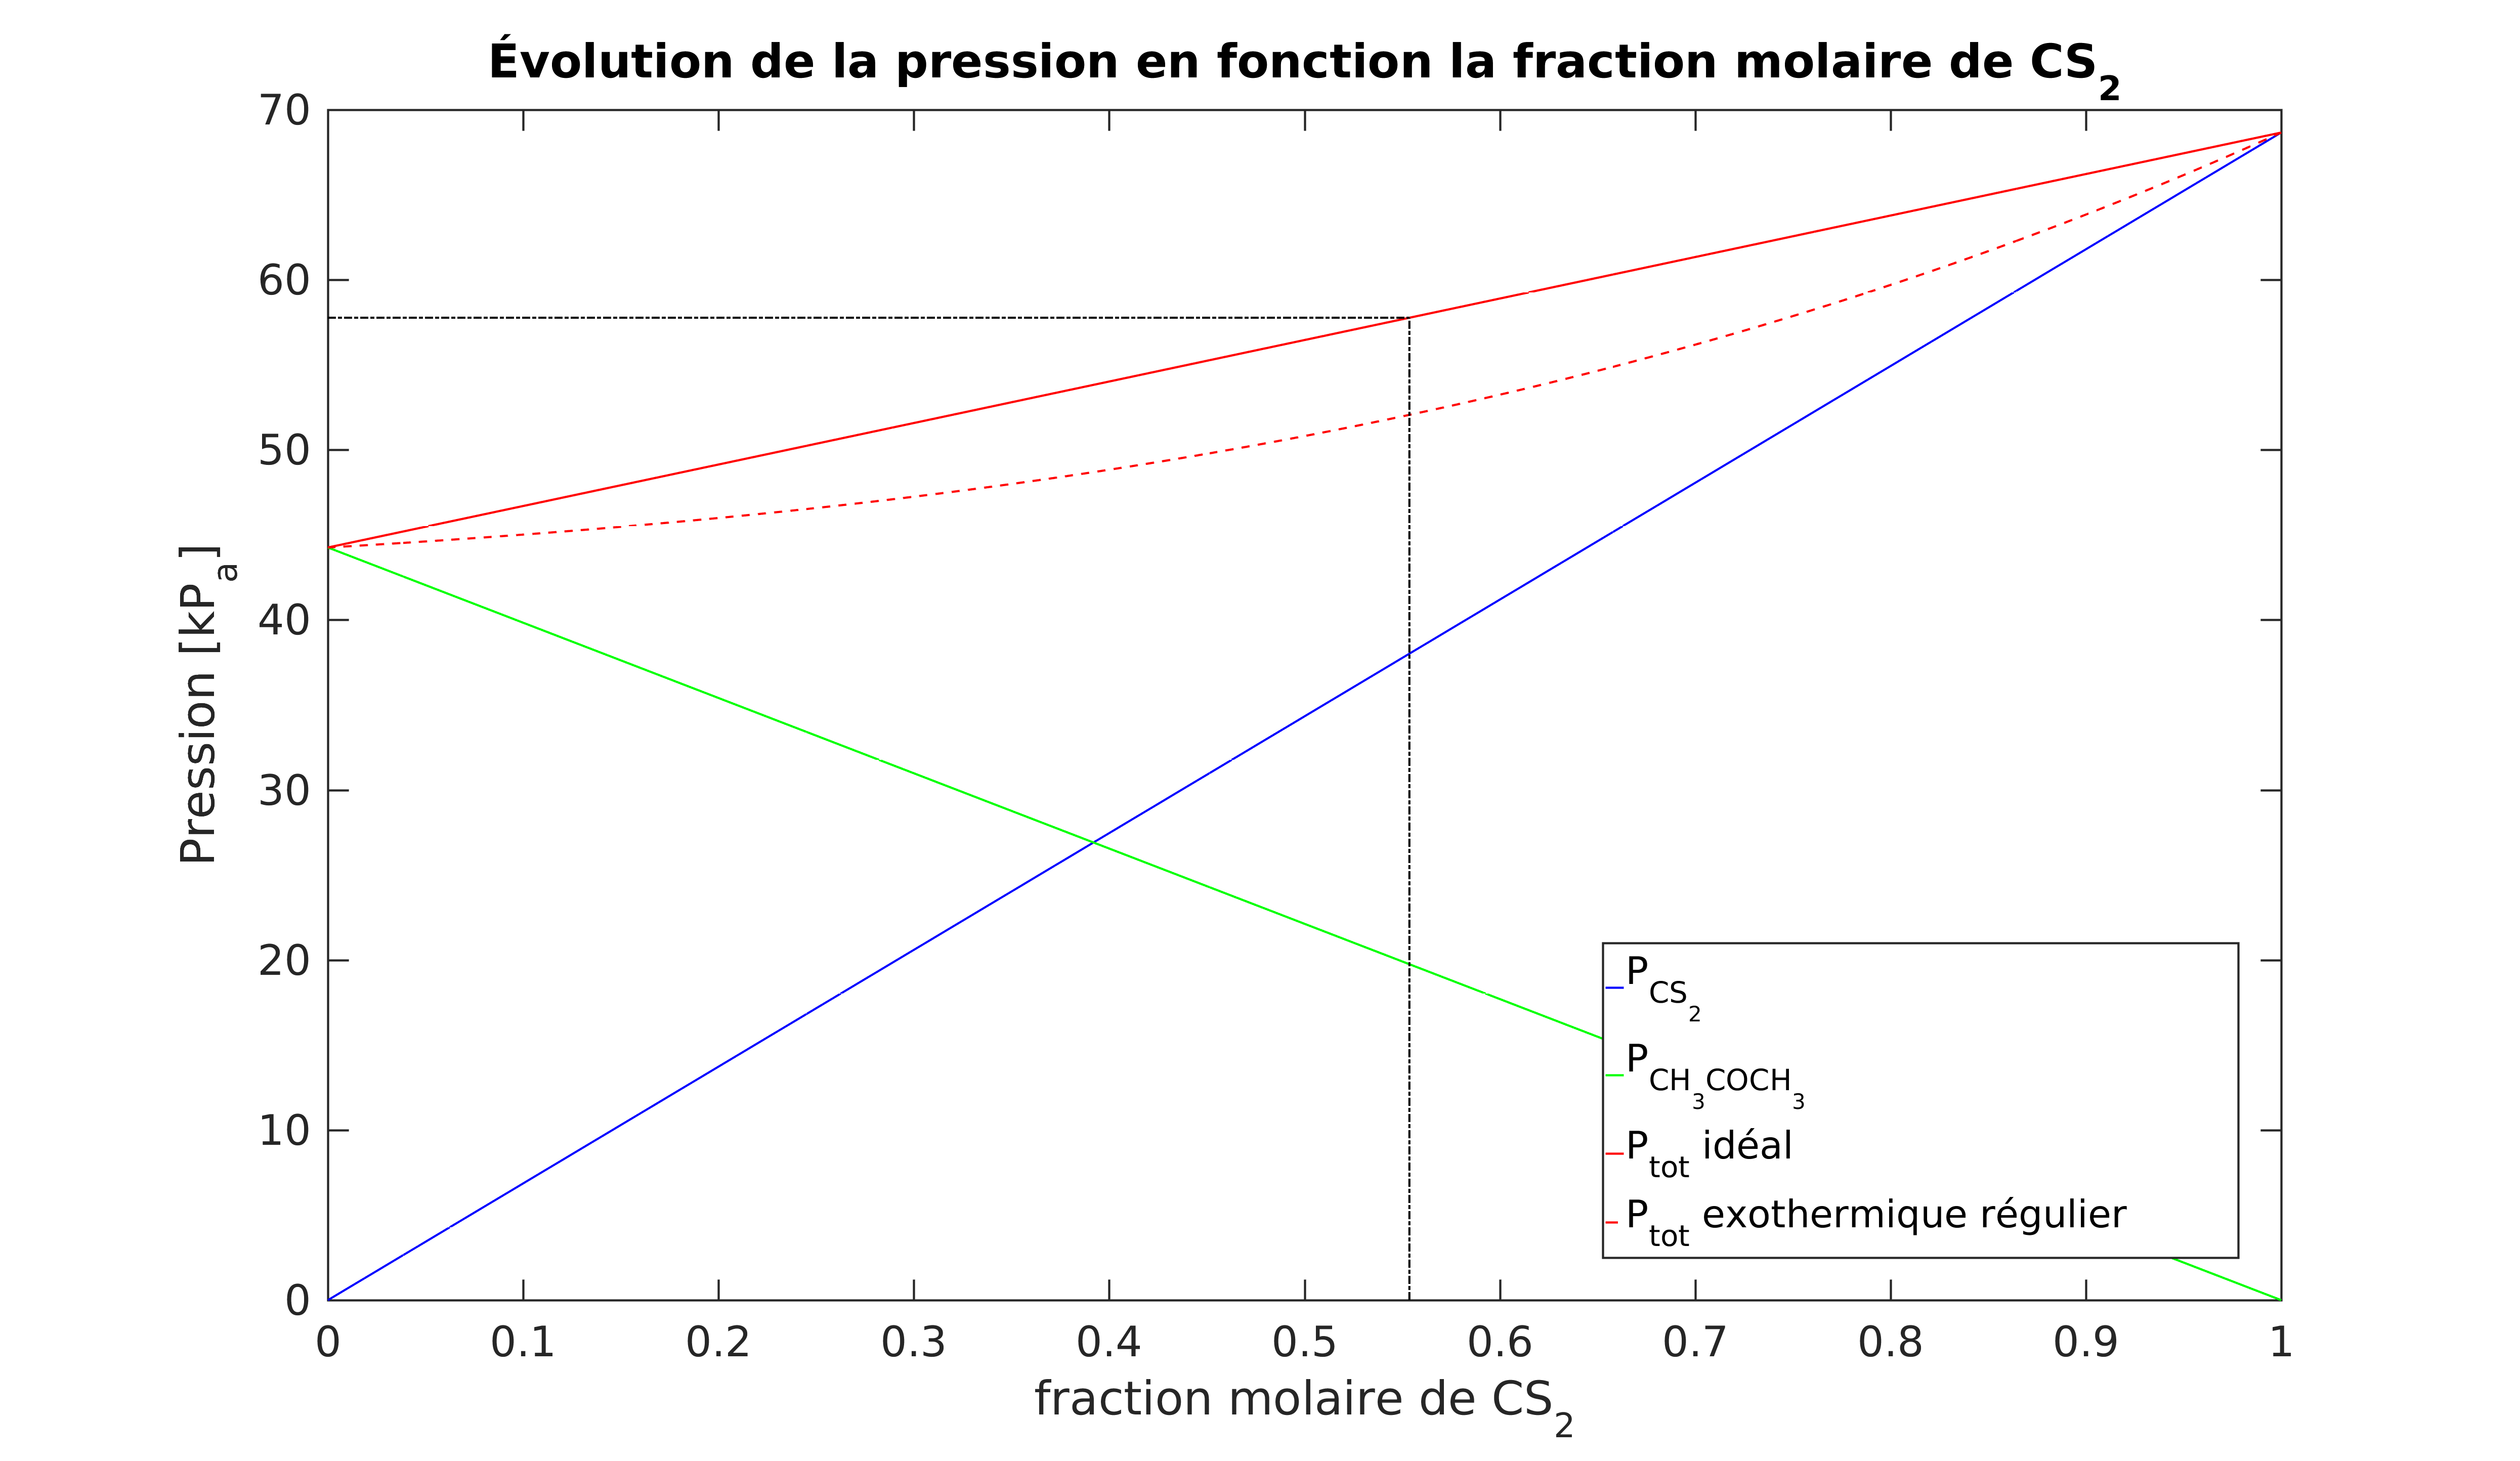
\includegraphics[scale=0.8]{Pression.png}
	\end{solfig}
	Pour une réaction exothermique $\Gamma \leq1$
	
\end{solution}

\section{Question 3}
Refroidir un gaz pendant sa compression permet de réduire le travail apporté. Ce concept peut être appliqué aux turbines à gaz stationnaires en insérant un refroidissement intermédiaire pendant l'étape de compression. Dans ce cas le cycle complet composé des transformation réversibles suivantes:

\begin{enumerate}
	\item 1--2: Compression isentropique
	\item 2--3: Refroidissement intermédiaire isobare
	\item 3--4: Compression isentropique
	\item 4--5: apport de chaleur isobare
	\item 5--6: détente isentropique
	\item 6--1:refroidissement isobare
\end{enumerate}
On vous propose de caractériser ce cycle dans le cadre des systèmes fermés. Le cycle est parcouru par un gaz assimilé à de l'air (gaz parfait) dont les propriétés thermiques sont telle que $\gamma = 1.3$. Le rapport de compression total est de 30. La pression intermédiaire (états 2 et 3) est choisie de telle manière à obtenir des travaux de compression identiques pour les transformations 1--2 et 3--4. Le refroidissement intermédiaire est supposé parfait $(T_3 = T_1)$. La température maximale du cycle est de $\SI{1500}{\kelvin}$.

Sur base de ces valeurs, on vous demande de
\begin{enumerate}
	\item compléter le tableau ci-dessous
	\item calculer le travail net du cycle
	\item calculer le rendement du cycle
\end{enumerate}

\begin{center}
	\begin{tabular}{|c|c|c|c|c|}
		\hline
		&p$[\si{\bar}]$&$T[\si{\kelvin}]$&$V[\si{\meter^3}]$&$S-S_1 [\SI{}{\joule\per\kelvin}]$\\
		\hline
		1&1&300&0.002&\\
		\hline
		2&&&&\\
		\hline
		3&&&&\\
		\hline
		4&&&&\\
		\hline
		5&&&&\\
		\hline
		6&&&&\\
		\hline
	\end{tabular}
\end{center}


\begin{solution}
	Commençons par remplir le tableau avec les autres données:
	\begin{center}
		\begin{tabular}{|c|c|c|c|c|}
			\hline
			&p$[\si{\bar}]$&$T[\si{\kelvin}]$&$V[\si{\meter^3}]$&$S-S_1 [\SI{}{\joule\per\kelvin}]$\\
			\hline
			1&1&300&0.002&0\\
			\hline
			2&$p_2$&$T_2$&$V_2$&0\\
			\hline
			3&$p_2$&300&$V_3$&$S_3$\\
			\hline
			4&$p_4$&$T_4$&$6.6*10^{-5}$&$S_3$\\
			\hline
			5&$p_4$&1500&$V_5$&$S_5$\\
			\hline
			6&1&$T_6$&$V_6$&$S_5$\\
			\hline
		\end{tabular}
	\end{center}
	Calculons la masse d'air présente:
	
	$$m = \frac{P_1 V_1}{R^* T_1} = \SI{2.32}{\gram} $$
	
	$\gamma$ nous étant donné, il nous faut recalculer $C_p$ et $C_v$:
	$$\gamma = \frac{C_p}{C_v} = \frac{mR^* + C_v}{C_v}$$
	$$C_v = \frac{mR^*}{\gamma -1} = 2.2222 $$
	$$C_p = C_V + mR^* = 2.888$$
	
	Attention $C_v$ et $C_p$ sont calculé en $\si{\joule\per\kelvin}$ 
	
	Si on considère uniquement nos colonnes p et V nous avons comme équation
	
	\begin{align}
		P_1V_1^{\gamma} &= P_2V_2^{\gamma}\\
		P_2V_3^{\gamma} &= P_4V_4^{\gamma}\\
		P_4V_5^{\gamma} &= P_6V_6^{\gamma}\\
		P_2V_3&= n R T_{3}\\
		P_4V_5&= nR T_{5}\\
		\frac{P_2V_2-P_1 V_1}{\gamma -1} &= \frac{P_4V_4-P_2 V_3}{\gamma -1}
	\end{align}
	La 6$^{ème}$ équation vient de :
	$$ W_{1-2} = W_{3-4}$$
	
	(6) peut se réécrire comme:
	$$ \frac{P_2V_2-nR^*T_1}{\gamma -1} = \frac{P_4V_4-nR^*T_3}{\gamma -1}$$
	$$P_2V_2 = P_4V_4 $$
	
	En prenant (1), (2), (4) et (6) nous avons 4 équations à 4 inconnues: $P_2 V_2 V_3 P_4$
	\begin{align*}
		V_3 &= \frac{mR^*T_3}{P_2}\\
		V_2 &= \left(\frac{P_1V_1^{\gamma}}{P2} \right)^{\cfrac{1}{\gamma}}\\
		P_4 &= \frac{P_2V_2}{V_4}\\
		P_2V_3^{\gamma} &= P_4V_4^{\gamma}\\
		P_2 * \left(\frac{mR^*T_3}{P_2} \right)^{\gamma}&=\frac{P_2}{V_4} \left(\frac{P_1V_1^{\gamma}}{P2} \right)^{\cfrac{1}{\gamma}} V_4^{\gamma}\\
		P_2^{\frac{1-\gamma^2}{\gamma}}	&=\frac{P_1^{\frac{1}{\gamma}}V_1 V_4^{\gamma - 1}}{(mR^*T_3)^{\gamma}} = 7.999*10^{-4}\\
		P_2&=\SI{6.84}{\bar}
	\end{align*}
	A partir d'ici on peut retrouver nos autres inconnues avec les relations
	
	\begin{center}
		\begin{tabular}{|c|c|c|c|c|}
			\hline
			&p$[\si{\bar}]$&$T[\si{\kelvin}]$&$V[\si{\meter^3}]$&$S-S_1 [\SI{}{\joule\per\kelvin}]$\\
			\hline
			1&1&300&0.002&0\\
			\hline
			2&6.84&468&$4.55*10^{-4}$&0\\
			\hline
			3&6.84&300&$2.93*10^{-4}$&$S_3$\\
			\hline
			4&46.8&468&$6.6*10^{-5}$&$S_3$\\
			\hline
			5&46.8&1500&$2.14*10^{-4}$&$S_5$\\
			\hline
			6&1&618&0.00412&$S_5$\\
			\hline
		\end{tabular}
	\end{center}
	
	$$S_3 = mc_p\ln(\frac{T_3}{T_2}) = -1.28 $$
	$$S_5 =S_3 + mc_p\ln(\frac{T_5}{T_4}) = -1.28 +3.36 = 2.08 $$
	Attention $c_p$ est exprimé en $\si{\joule\per\kelvin\per\kilogram}$
	
	$$W_{tot} = W_{1-2} + W_{2-3} + W_{3-4} +W_{4-5} +W_{5-6} +W_{6-1}$$
	$$W_{tot}=2* \frac{mR^*T_2 - mR^*T1}{\gamma -1} + \frac{mR^*T_6 - mR^*T5}{\gamma -1} - P_2 (V_3-V_2)- P_4 (V_5-V_4)- P_1 (V_6-V_1) = -1578$$
	
	$$Q_1 = C_p \Delta T = -485$$
	$$Q_2= C_p \Delta T = 2981$$
	$$Q_3= C_p \Delta T = -918$$
	
	$$\eta = \frac{Q_1+Q_2+Q_3}{Q_2} =  0.53$$
	
\end{solution}
\section{Question 4}
Dans le cadre de l'étude de la thermodynamique, nous avons abordé la seconde expérience de Joule sur l'expansion libre d'un gaz. Concernant cette expériences ,on vous demande

\begin{enumerate}
	\item d'énoncer succinctement l'objectif poursuivi
	\item d'exposer (en vous aidant d'un schéma) le principe de l'installation expérimentale utilisée
	\item de déduire mathématiquement la conséquence du résultat de l'expérience
	\item de commenter la généralité du résultat obtenu par Joule.
\end{enumerate}

\begin{solution}
	Cf Syllabus 
\end{solution}

\section{QCM}
\begin{enumerate}
	\item A $\SI{300}{\kelvin}$ et à pression atmosphérique, quelle est la vitesse quadratique moyenne des molécules de dioxyde de carbone ?
	\begin{align*}
		&\SI{380}{\meter\per\second}
		&\SI{11}{\meter\per\second}&
		&\SI{337}{\meter\per\second}&
		&\SI{412}{\meter\per\second}&
		&\SI{505}{\meter\per\second}
	\end{align*}
	
	\item Une machine frigorifique travaille selon un cycle de carnot inversé entre une température extérieur de $\SI{30}{\celsius}$ et une température intérieure de $\SI{5}{\celsius}$.Quel est le coefficient de performance de cette machine?
	\begin{align*}
		&3.2
		&12.1&
		&11.1&
		&0.2&
		&1.2
	\end{align*}
	
	\item De l'hydrogène (gaz parfait aux propriétés constantes prises à température ambiante) est produit à $\SI{30}{\bar}$ et à température ambiante ($\SI{300}{\kelvin}$) via une électrolyse de l'eau. Afin de le stocker, on souhaite augmenter sa pression à $\SI{200}{\bar}$. La compression se fait de manière isentropique dans un turbocompresseur (système ouvert). Le débit d'hydrogène est de $\SI{100}{\gram \per \second}$. Quelle sera la puissance du compresseur ?
	\begin{align*}
		&\SI{224}{\kilo\watt}
		&\SI{22}{\kilo\watt}&
		&\SI{25}{\kilo\watt}&
		&\SI{314}{\kilo\watt}&
		&\SI{356}{\kilo\watt}
	\end{align*}
	
	\item Vous trouverez à la figure \ref{fig:solution} un graphe de la variation de l'énergie libre molaire avec la concentration. Laquelle des expressions suivantes n'est \textbf{pas} valable à la concentration $x_B$
	
	\begin{align*}
		&G_m^{A^{\circ}} < G_m^{B^{\circ}}
		& \mu_B > G_m^{B^{\circ}}&
		& \mu_A > G_m^{A^{\circ}}&
		&\mu_A <\mu_B&
		&\omega <0
	\end{align*}
	
	
	\item Une batterie rechargeable consiste en deux électrodes: une plaque d'or et une plaque de cuivre pour lesquelles les potentiels d'équilibre standard sont $\SI{1.5}{\volt}$ et $\SI{0.34}{\volt}$, respectivement. Quelle condition doivent respecter les concentrations en \ce{Au+++} et \ce{Cu++} auprès de chaque électrode pour que la différence de tension aux bornes de la batterie devienne supérieur à la force électromotrice standard de la batterie.
	
	\[
		[\ce{Cu++}]^3 < [\ce{Au+++}]^2\qquad
		[\ce{Cu++}]>0\text{ et }[\ce{Au+++}]>0\qquad
		[\ce{Au+++}]^3<[\ce{Cu++}]^2
	\]
	
	\begin{center}
			\begin{tabular}{cc}
			$[\ce{Au+++}]>[\ce{Cu++}]$&
			$[\ce{Au+++}]^3>[\ce{Cu++}]^2$
		\end{tabular}
	\end{center}

	\item Le grillage est un procédé  chimique exothermique qui permet de transformer des sulfures en oxydes, p.e. $2\ce{ZnS} +3\ce{O2} = 2\ce{ZnO} + 2\ce{SO2}$. Quelle est, à une température et une pression partielle d'\ce{O2} données, la condition à respecter dans un réacteur de grillage afin de diriger le procédé dans le bon sens ?
	\begin{align*}
		& p_{\ce{SO2}} > p_{\ce{O2}}
		& p_{\ce{SO2}} > p_{\ce{SO2},eq}&
		&p_{\ce{O2}} > p_{\ce{O2},eq}&
		&p_{\ce{SO2}} < p_{\ce{SO2},eq}&
		&p_{\ce{SO2}} <p_{\ce{O2}}
	\end{align*}
	
	\item Quelle expression parmi les suivantes n'est \textbf{pas} correcte ?
	
	\begin{align*}
		& (\fpart{H}{p})_S = V
		& (\fpart{U}{S})_V = T&
		&(\fpart{T}{V})_S = (\fpart{p}{S})_V&
		&(\fpart{T}{p})_S = (\fpart{V}{S})_p
	\end{align*}
	
	\item Afin de mesurer le débit d'eau dans une conduite de \SI{100}{\milli\meter} de diamètre, on réalise localement une contraction régulière avec un rapport de diamètre de 2. La chute de pression locale est mesurée à \SI{2000}{\pascal}. Quel est approximativement le débit dans la conduite ?
	\begin{align*}
		& \SI{800}{\litre\per\second}
		& \SI{1}{\kilogram\per\second}&
		& \SI{4}{\kilogram\per\second}&
		& \SI{8}{\kilogram\per\second}&
		& \SI{4000}{\litre\per\second}
	\end{align*}
	
	\item Quelle est la définition générale de l'activité d'un composant gazeux i ?
	
	\begin{align*}
		& \cfrac{p_i}{p_i^{\circ}}
		& p_i&
		& \cfrac{p_i}{p^{\circ}}&
		& p_i^{\circ}&
		& \cfrac{p}{p_i^{\circ}}
	\end{align*}
	
	\item Lequel des symboles ci-dessous est synonyme du potentiel chimique standard d'un composant i dans un mélange réactionnel ?
	
	\begin{align*}
		& \cfrac{dG}{dn_i}
		& G_{im}^{\circ}&
		&G^{i^{\circ}}&
		&G_{m}^{i^{\circ}}&
		&G_{i}^{\circ}
	\end{align*}
	
		\begin{figure}[!ht]
			\begin{center}
				\begin{tikzpicture}[xscale = 2.25,yscale=2]
				\draw [thick,->] (3,4) -- (3,0) -- (0,0) -- (0,3);
				\draw [dashed] (0,2.34) -- (3,3.34);
				\draw [domain=0:1,samples=200] plot (\x*3,93.2540*\x*\x*\x*\x -187.54*\x*\x*\x +115*\x*\x -20*\x+1.7);
				\draw [*-,dashed] (1.5,2.875) --(1.5,0);
				\draw (0,0)node[below]{0};
				\draw (3,0) node[below]{1};
				\draw (1.55,0) node[below]{$x_B$};
				\end{tikzpicture}
			\end{center}
			\caption{Variation de l'énergie libre molaire avec la concentration}
			\label{fig:solution}
		\end{figure}
	
\end{enumerate}
\begin{solution}
	\begin{enumerate}
		\item \SI{412}{\meter\per\second}
		\item 11.1
		\item \SI{314}{\kilo\watt}
		
		Il faut utiliser la formule d'un système ouvert et intégrer $vdp$ et non $pdv$
		\item $\omega < 0$
		\item$[\ce{Cu++}]^3 < [\ce{Au+++}]^2$
		\item$p_{\ce{SO2}} < p_{\ce{SO2},eq}$
		\item $(\fpart{T}{V})_S = (\fpart{p}{S})_V$
		\item  \SI{4}{\kilo\per\second}
		\item $\cfrac{p_i}{p_i^{\circ}}$
		\item $G_{im}^{\circ}$
	\end{enumerate}
\end{solution}

\end{document}
